\documentclass[11pt]{beamer}
\usepackage[utf8]{inputenc}
\usepackage[spanish]{babel}
\usepackage{amsmath}
\usepackage{amsfonts}
\usepackage{amssymb}
\usepackage{graphicx}
\usetheme{Copenhagen}
\usepackage{multicol}
\addtobeamertemplate{navigation symbols}{}{%
	\usebeamerfont{footline}%
	\usebeamercolor[fg]{footline}%
	\hspace{1em}%
	\insertframenumber/\inserttotalframenumber
	\setbeamercolor{footline}{fg=black}
	\setbeamerfont{footline}{series=\bfseries}
}

\begin{document}
\author{Hiram Ernesto Damian \\
\textit{Avance de tesis, Programa de Maestria (DIFUS)\\ 
	Dr. José Benitez Rubio (D), Dr. Jorge Gaspar Armenta (T), Dr. Marcelino Barboza Flores}}
\title{Estudio del proceso de producción del bosón de Higgs  en asociación con un solo quark de tipo top en colisiones protón-protón del LHC} 

	%\subtitle{}
	\logo{
\includegraphics[scale=0.08]{unison-logo.png}}
	\institute{Universidad de Sonora}
	\date{3 de Diciembre de 2018}
	%\subject{}
	%\setbeamercovered{transparent}
	%\setbeamertemplate{navigation symbols}{}
	\begin{frame}[plain]
	\maketitle
	\begin{center}
		\begin{figure}
		
\includegraphics[scale=0.18]{unison-logo.png}
		\end{figure}
	\end{center} 
\end{frame}
\begin{frame}
\frametitle{Tabla de contenido}
\tableofcontents
\end{frame}

\begin{frame}
\section{Introducci\'on}
\subsection{Objetivo general}
\frametitle{Objetivo general}
\begin{itemize}
	\item Mediante este proyecto se investigará la producción del bosón de Higgs en asociación
	con un solo quark de tipo top (tH) en colisiones protón-protón con el experimento CMS
	del LHC. Este mecanismo de producción del bosón de Higgs no ha sido observado antes
	por ningún experimento.\\
	
	\item El entender la producción del bosón de Higgs, así como sus
	decaimientos son una parte importante del programa de física de los experimentos del
	laboratorio internacional CERN que intenta completar las pruebas para verificar el
	Modelo Estándar, la teoría de las partículas fundamentales.
\end{itemize}
\end{frame}

\begin{frame}
\begin{center}
	\begin{figure}[ht]
		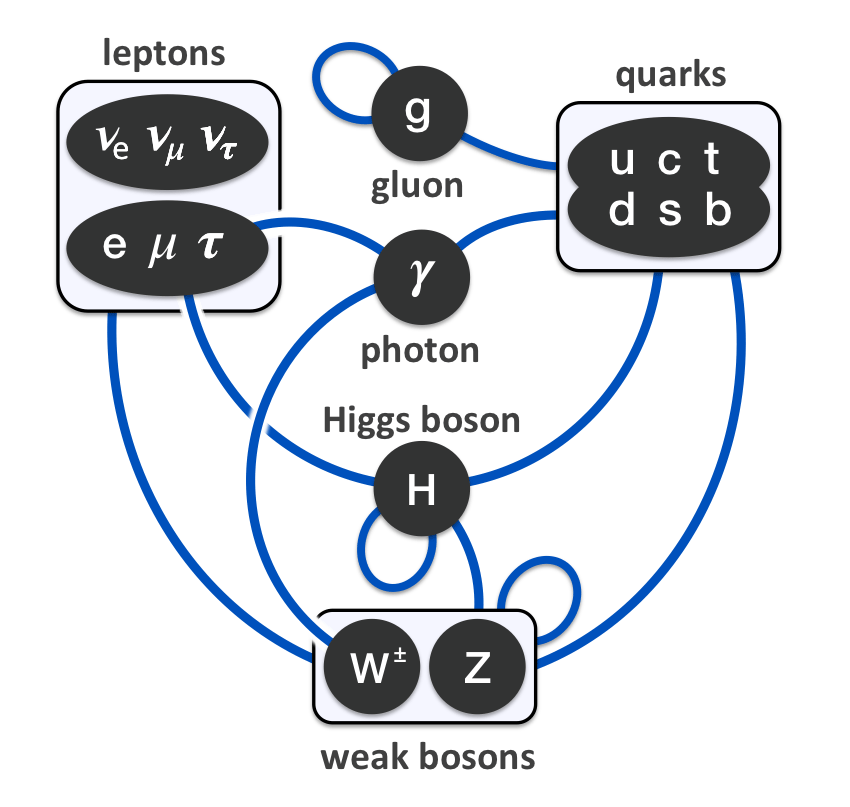
\includegraphics[scale=0.24]{sm.png}
	\end{figure}
\end{center}
\end{frame}


\begin{frame}
\frametitle{Mecanismo de producci\'on}
\begin{center}
	\begin{figure}
		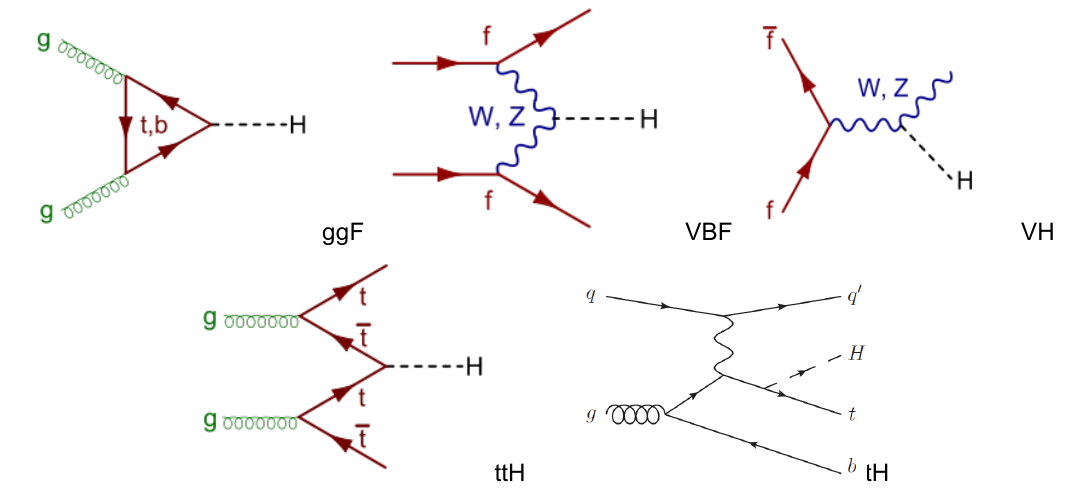
\includegraphics[width=\linewidth]{pg.png}
		\caption{canales de producci\'on del bos\'on de Higgs}
	\end{figure}
\end{center}
\end{frame}



\begin{frame}
\frametitle{Mecanismo de producci\'on}
\begin{center}
	\begin{figure}
		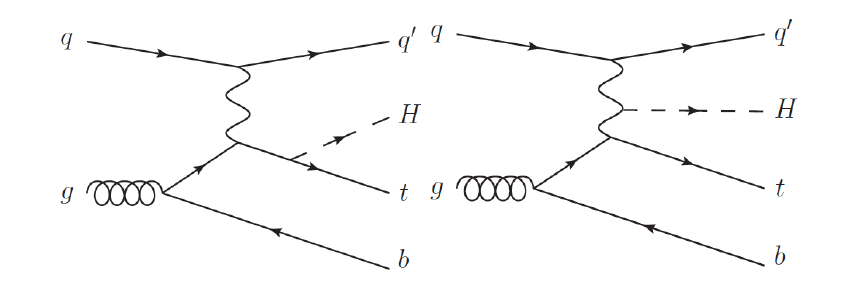
\includegraphics[width=\linewidth]{tq.png}
		\caption{canales de producci\'on \textsc{tH}}
	\end{figure}
\end{center}	
\end{frame}

\begin{frame}
\section{Motivaci\'on}
\frametitle{Motivaci\'on}

\begin{itemize}
	\item Medici\'on de acoplamientos es esencial para establecer la naturaleza del Higgs
	\item La exploraci\'on de producci\'on de Higgs en el canal Th es tema relativamente nuevo. 
	\item El estudio de tHq explora el signo relativo de  top-Higgs y W-Higgs
	\item Mediciones de CMS y ATLAS son compatibles con SM.
	\item peque\~nas desviaciones de las predicciones del SM podr\'an estar asociadas con f\'isica mas all\'a del modelo est\'andar (BSM)
\end{itemize}
\end{frame}





\begin{frame}
\frametitle{Canales de producci\'on de Higgs}
\begin{center}
\begin{figure}
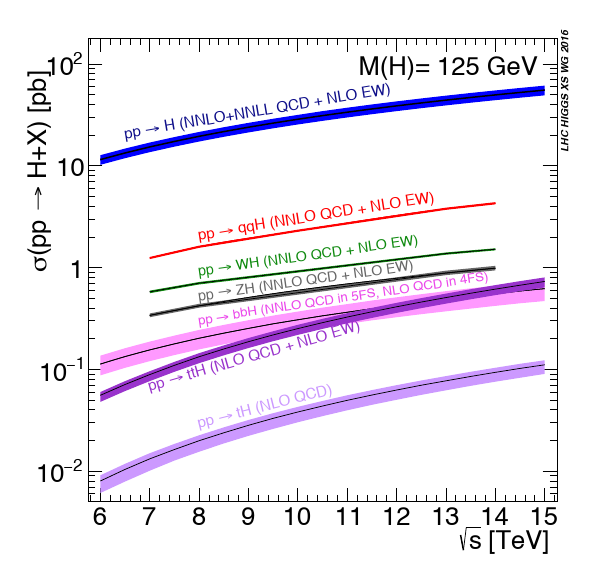
\includegraphics[width=6cm]{yuk.png}
\end{figure}
\end{center}
\end{frame}

\begin{frame}
\frametitle{Topología de eventos tH}
\subsection{Topología de eventos tH}
\begin{multicols}{2}
\scriptsize{
%Un jet es un peque\~no cono de hadrones y otras part\'iculas producidas por hadronizaci\'on de un quark y un glu\'on.}\\

\vspace{3mm}
%\scriptsize{
%	Hadronizaci\'on es el proceso de la formaci\'on de hadrones de quarks y gluones. Ocurre despu\'es de colisiones de alta energ\'ia en un colisionador de part\'iculas donde los quark y gluones son creados. Por el confinamiento del color, \'estos no pueden existir individualmente.\\
%\vspace{3mm}
%Los leptones son part\'iculas elementales en las cuales poseen spin $1/2$ que no experimentan interacci\'on fuerte. }
Las caracter\'isticas de la se\~nal tHq:
\begin{itemize}
\item un jet ligero hacia adelante 

\item un b-jet y un bos\'on W de decaimiento del top con $W\rightarrow l \nu$ 

\item Un bos\'on Higgs 
\end{itemize}
}
\columnbreak
\begin{figure}
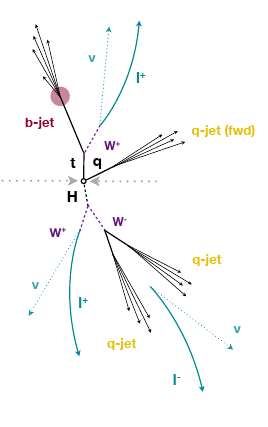
\includegraphics[scale=0.5]{jet.png}
\end{figure}
\end{multicols}
\end{frame}



\begin{frame}
\section{Exploraci\'on de los datos de CMS}
\frametitle{Exploraci\'on de los datos de CMS}
\footnotesize{
\begin{itemize}
\item El análisis explota se\~nales con dos leptones de mismo signos iguales y utiliza la muestra de datos recopilada de 2016 $ \sqrt{s} $ = 13 TeV que corresponde a una luminosidad integrada de 35.9 $ fb^{-1} $.
\item En este análisis, los métodos de reconstrucciónes hacen dif\'icil distingir  entre tH y t\={t}H porque
la sección transversal efectiva de t\={t} H es mucho más alta que tH y algunos eventos pasan las selecciones
diseñado para tH, la fracción de eventos de tH sobre tH + t\={t}H es 5 $\%$.

\end{itemize}
}
\end{frame}

\begin{frame}
\begin{center}
\begin{figure}
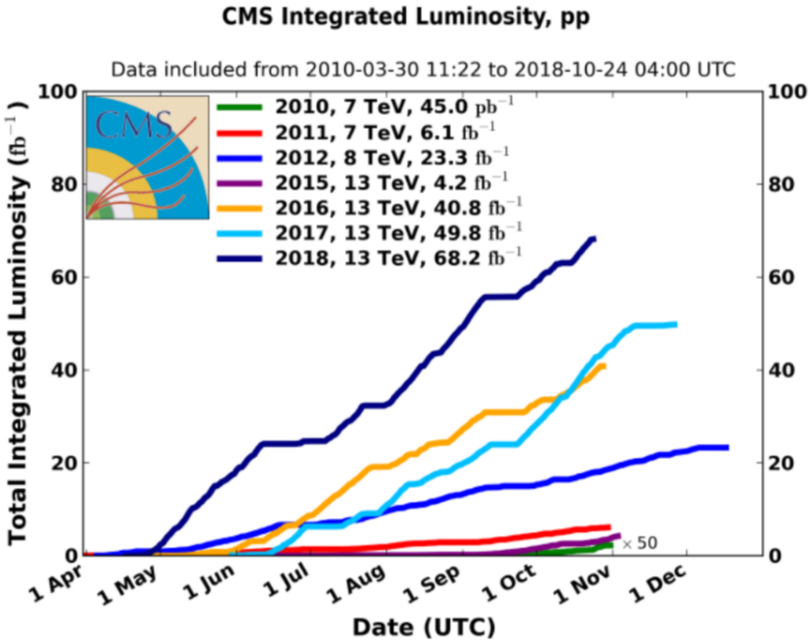
\includegraphics[width=6cm]{cms_lumi.png}
\caption{Datos acumulados en CMS}
\end{figure}
\end{center}
\end{frame}

\begin{frame}
\section{Selecci\'on de eventos}
\frametitle{Selecci\'on de eventos}


\begin{itemize}
\scriptsize{
\item Los eventos se seleccionan aquellos que contienen dos leptones ($\mu \mu$) con el mismo signo.
\item  Al utilizar un canal de dos leptones con el mismo signo, se seleccionan mayormente $ H \rightarrow WW $. También se incluyen las contribuciones de $ H \rightarrow \tau \tau $ ,$ H \rightarrow ZZ $. 
\item La principal estrategia de análisis es obtener una selección de eventos compatibles con ciertas características de la señal. Se requiere:} 

\begin{itemize}
\tiny{
	\item momento transversal $p_T> 25$ y $15$ GeV, para los muones.
	\item un jet delantero con  $p_T > 40$ GeV, $|\eta| > 2.4$ 
	\item uno o m\'as b-jets con ($|\eta| < 2.4$) %$\eta$  es pseudorapidez., Csv es un algoritmo seleccionador de b jets 
}
\end{itemize}

\end{itemize}

\end{frame}

\begin{frame}
\subsection{Discriminaci\'on de se\~nal usando BDT}
\frametitle{BDT:Boosted decision tree}
\begin{multicols}{2}

\begin{itemize}
\tiny{
\item Un árbol de decisión toma un conjunto de características de entrada y divide los datos de entrada
recursivamente basado en esas características.
\item El boosting es un método para combinar muchos aprendices débiles (árboles) en un clasificador fuerte.
\item Algunas variables para BDT
}
\begin{itemize}
\tiny{
	\item  momento transversal  de los muones
	\item N\'umero de  b-jets con $|\eta| < 2.4$
	\item N\'umero de  light jets 
}
\end{itemize}

\end{itemize}

\columnbreak
\begin{center}
	\begin{figure}
		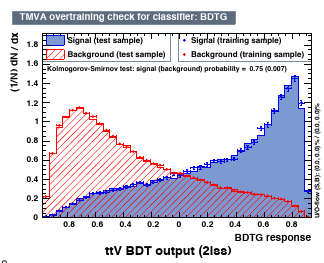
\includegraphics[scale=0.5]{sk.png}
	\end{figure}
	
\end{center}
\end{multicols}
\end{frame}

\begin{frame}
\frametitle{Incertidumbres sistem\'aticas}
Valores de las Incertidumbres sistem\'aticas en la normalizaci\'on de los ruidos (Backgrounds):
\begin{itemize}
	\item t\=tW  : 12$\%$  
	\item t\=tZ : 10$\%$ 
	\item tZ,VVV,$W^{\pm}$ $W^{\pm}$:  50$\%$  
	\item WZ: 50$\%$    
	\item non-prompt lepton (Fakes) : 50$\%$ 
\end{itemize}

\end{frame}



\begin{frame}
\frametitle{Herramientas de an\'alisis}
\scriptsize{
\begin{itemize}
\item  \textbf{ROOT} es un kit de herramientas de software científico modular. Proporciona todas las funcionalidades necesarias para tratar el procesamiento de grandes datos, el análisis estadístico, la visualización y el almacenamiento. Está escrito principalmente en C ++ pero integrado con otros lenguajes como Python y R.

\item La biblioteca \textbf{RooFit} proporciona un conjunto de herramientas para modelar la distribución esperada de eventos en un análisis. Los modelos se pueden usar para realizar ajustes y  producir gráficos  para diversos estudios.

\end{itemize}
}
\end{frame}

%\begin{frame}
%\LARGE{Non prompt leptons}:\\
%\scriptsize{
%	\begin{itemize}
%		\item un prompt lepton es un lepton que se origina en la colisión principal que tiene lugar en el evento, como un producto directo de la descomposición en particular que está buscando. Un análisis en busca de un estado final particular que contenga leptons realmente está buscando prompt lepton. 
%		\item Los non prompt leptons  llegan más tarde: ya sea a través de la descomposición de los quarks hadronizados (los llamados jets), o como una "miss-id".
%		\item También podría darse el caso de que debido a una se\~nal de jet  particular o una falla en una parte del detector, un jet  se reconstruya como un lepton. Estos leptons "mis-ID" o "falsos" también se consideran non prompt .
%	\end{itemize}
%}
%\end{frame}


\begin{frame}
\section{Resultados}
\frametitle{Resultados}
\begin{center}
	\begin{minipage}{0.5\textwidth}
		\centering
		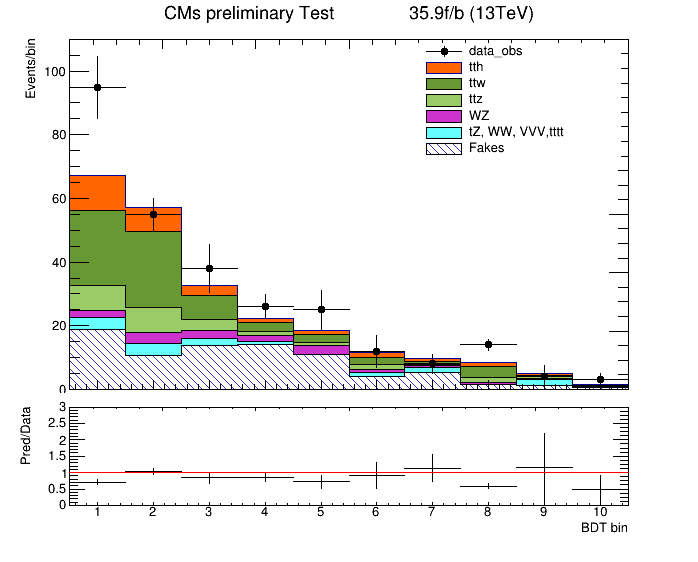
\includegraphics[width=.95\linewidth]{hist-function.png}\label{Fig:Data1}
	\end{minipage}\hfill
	\begin{minipage}{0.5\textwidth}
		\centering
		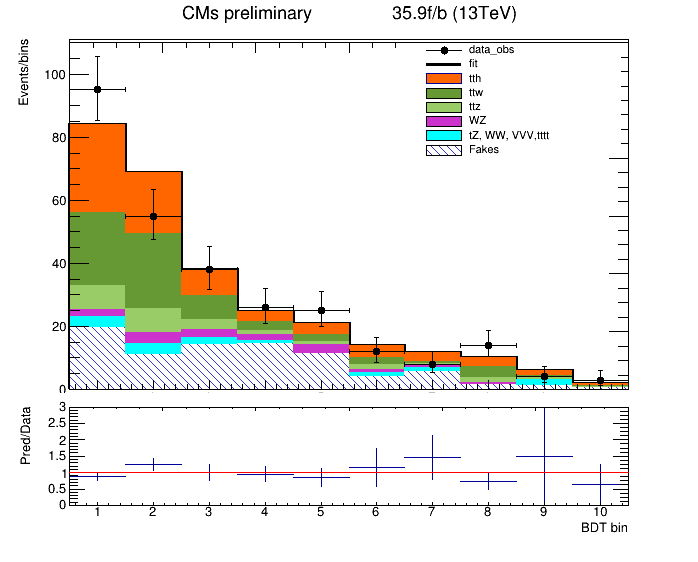
\includegraphics[width=.95\linewidth]{histofit-constrain.png}\label{Fig:Data2}
	\end{minipage}
	\begin{footnotesize}
		Figura 1. Pre-fit and post-fit BDT distributions.
	\end{footnotesize}
\end{center}
\end{frame}



\begin{frame}
\frametitle{Resultados}
\begin{center}
	
	Tabla 2. Tabla de  n\'umero de eventos despu\'es de la selecci\'on y el ajuste para el canal de producci\'on $\mu\mu$ correspondiente a 35.9fb$^{-1}$ de luminosidad.\\ 
	
\scriptsize{
	\begin{tabular}{ccc}
		\hline
		Process & Pre-fit & Post-fit \\
		\hline
		t \={t} W$^{\pm}$ & 68.02 $\pm$ 34.01 &67.54 $\pm$ 8.27 \\
		t\={t}Z &	25.88$ \pm$ 12.94 &  25.83 $\pm$ 2.78\\
		WZ 	&	15.07 $\pm$ 7.53 & 15.44$\pm$ 7.06 \\
		tZ,VVV,t\={t} t\={t} ,$W^{\pm}$ $W^{\pm}$ & 15.73$\pm$ 7.86 &  20.56$\pm$6.32\\
		non -prompt    &   80.93 $\pm$ 40.46 & 75.85$\pm$ 6.77\\
		t\={t}h+th 		&	28.65 & 69.70$\pm$ 22.45\\
		\textbf{Data}\quad 280 &	&  
	\end{tabular}
}
\end{center}

\end{frame}

%\begin{frame}
%\begin{center}
%\scriptsize{Tabla 3. Valores de las incertidumbres para los ruidos y se\~nales.
%\begin{tabular}{c|c|c|c}
%	\hline
% & alpha-sample &ERROR & Events \\
% (ttz) & -0.01981 &  9.98956e-01 & 25.3726 \\  
% (non-prompt)& -0.15688 & 2.09273e-01 &   68.2414\\ 
% (ttw)& -0.05615 & 9.61843e-01 & 64.2085\\
% (Wz)& 0.04914 & 9.36848e-01 &  15.8140\\
% (tz) &  0.61373  & 8.03989e-01 &  25.3876  \\

%Lumi=1.0
%mu= 2.4328
%thq=69.705
%\end{tabular} }
%\end{center}
%\end{frame}


\begin{frame}
\section{Actividades}
\frametitle{Actividades realizadas}
\scriptsize{
\textbf{Semestre 2018-2}
\begin{itemize}
	\item curso optativo de F\'isica de part\'iculas.
	\item Participaci\'on en XVIII Mexican School of Particles and Fields 2018, realizada en Hermosillo,Sonora. 

	\item El estudio de los datos actuales y proyecciones para las diferentes fases del
	LHC, y con ello generar ajustes.
	\item Aprendizaje del lenguaje ROOT para an\'alisis y ajuste de datos.
\end{itemize}
\vspace{4mm}
\textbf{Semestre 2019-1}
\begin{itemize}
	\item Continuar aprendizaje de las particulas elementales, su produccion y decamientos
	\item Finalizar analysis estadistico de los datos
	\item Escribir tesis
\end{itemize}
}
\end{frame}



\begin{frame}
\section{Resumen}
\frametitle{Resumen}
\begin{itemize}
\item Se ha estudiado los datos del canal de $\mu \mu$ para la producción de th + t\=th.
\item Al usar los datos de 2016 del experimento CMS, y luego de hacer un ajuste con las herramientas de Root y Roofit, obtenemos una cantidad de  eventos de se\~nal de  70$\pm$ 22 con una significancia  aproximada de $3\sigma$.
\item Se planea tambi\'en estudiar la sensibilidad a tH, no solo la suma t\=tH+tH, aplicando ajustes donde se separan los 2. 
\item  Se agregar\'an siste'aticos que toman en cuenta variaciones en las distribuciones (shape systematics).
\end{itemize}	
\end{frame}



\begin{thebibliography}{99}
\begin{frame}
\section{Referencias}
\frametitle{Referencias}
\bibliographystyle{amsalpha}

	%\bibitem{c1}The CMS collaboration, \"Observation of ttH production”, PRL 120 (2018) 231801
	\bibitem{c5}\"Measurements of the Higgs boson production and decay rates and constraints on
	its couplings from a combined ATLAS and CMS analysis of the LHC pp collision
	data at $\sqrt{s}$ = 7 and 8 TeV”, J. High Energy Phys. 08 (2016) 045.
	\bibitem{c2}The ATLAS Collaboration, \"Search for produced in association with top quarks
	and constraints on the Yukawa coupling between the top quark and the Higgs
	boson using data taken at 7 TeV and 8 TeV with the ATLAS detector “, Physics
	Letters B 740 (2015) 222-242
\end{frame}

\begin{frame}
	\bibitem{c3}The CMS collaboration, "Search for production of a Higgs boson and a single top
quark in multilepton final states in proton collisions at 13 TeV”, CMS-PAS-HIG-17-
005
		\bibitem{c4}The CMS collaboration, \"Search for $H \rightarrow bb$ in association with a single top quark
	as a test of Higgs boson couplings at $\sqrt{s}= 13$ TeV”, CMS-PAS-HIG-16-019
	\bibitem{incropera} 
	Griffiths, D.  {\em Introduction to elementary Particles} John Willey \& sons. 
	Second edition, 2008
	\bibitem{usd} Cowan, G {\em Stadistical data analysis} Oxford University Press 1998.
	\bibitem{gross} Gross, F. "Relativistic Quantum Mechanics and field theory", Willey 1994. 
\end{frame}
\end{thebibliography}
\end{document}